% =====================================================================
% MuGate -- Springer LNCS format (llncs class, splncs04 bibliography style).
% Compile with pdfLaTeX + BibTeX, e.g. on Overleaf using the official
% "Springer Lecture Notes in Computer Science" template (provides llncs.cls
% and splncs04.bst). All numbers come from numbers.tex and tables/*.tex,
% which are generated from results/summary.json by mugate/make_tables.py.
% =====================================================================
\documentclass[runningheads]{llncs}
\usepackage[T1]{fontenc}
\usepackage{graphicx}
\usepackage{booktabs}
\usepackage{amsmath,amssymb}
\usepackage{array}
\usepackage{tikz}
\usetikzlibrary{shapes.geometric,arrows.meta,positioning,calc}
\usepackage{xcolor}
\usepackage[hidelinks]{hyperref}
\usepackage{url}
% Auto-generated by mugate/make_tables.py from results/summary.json. Do not edit by hand.
\newcommand{\nTasks}{50}
\newcommand{\nMut}{883}
\newcommand{\nGateMut}{282}
\newcommand{\nHeldMut}{601}
\newcommand{\nKillable}{833}
\newcommand{\pctKillable}{94.3}
\newcommand{\nSurv}{52}
\newcommand{\nEqAudit}{36}
\newcommand{\nEqPre}{14}
\newcommand{\nSurvKillable}{2}
\newcommand{\msHuman}{97.6}
\newcommand{\killedHuman}{813}
\newcommand{\loHuman}{95.6}
\newcommand{\hiHuman}{99.1}
\newcommand{\rawHuman}{92.1}
\newcommand{\msGateGrpHuman}{98.2}
\newcommand{\msHeldGrpHuman}{97.3}
\newcommand{\deltaHuman}{\ensuremath{-0.8}}
\newcommand{\perfectHuman}{39}
\newcommand{\msVanilla}{96.3}
\newcommand{\killedVanilla}{802}
\newcommand{\loVanilla}{93.3}
\newcommand{\hiVanilla}{99.0}
\newcommand{\rawVanilla}{90.8}
\newcommand{\msGateGrpVanilla}{97.4}
\newcommand{\msHeldGrpVanilla}{95.7}
\newcommand{\deltaVanilla}{\ensuremath{-1.7}}
\newcommand{\perfectVanilla}{41}
\newcommand{\msBlind}{98.3}
\newcommand{\killedBlind}{819}
\newcommand{\loBlind}{96.6}
\newcommand{\hiBlind}{99.7}
\newcommand{\rawBlind}{92.8}
\newcommand{\msGateGrpBlind}{98.2}
\newcommand{\msHeldGrpBlind}{98.4}
\newcommand{\deltaBlind}{\ensuremath{+0.2}}
\newcommand{\perfectBlind}{45}
\newcommand{\msGate}{97.6}
\newcommand{\killedGate}{813}
\newcommand{\loGate}{94.8}
\newcommand{\hiGate}{99.5}
\newcommand{\rawGate}{92.1}
\newcommand{\msGateGrpGate}{100.0}
\newcommand{\msHeldGrpGate}{96.4}
\newcommand{\deltaGate}{\ensuremath{-3.6}}
\newcommand{\perfectGate}{42}
\newcommand{\dVanHum}{\ensuremath{-1.3}}
\newcommand{\ciLoVanHum}{\ensuremath{-4.7}}
\newcommand{\ciHiVanHum}{\ensuremath{+1.8}}
\newcommand{\pWVanHum}{0.624}
\newcommand{\pSVanHum}{0.727}
\newcommand{\upVanHum}{5}
\newcommand{\downVanHum}{3}
\newcommand{\onlyAVanHum}{10}
\newcommand{\onlyBVanHum}{21}
\newcommand{\dBliVan}{\ensuremath{+2.0}}
\newcommand{\ciLoBliVan}{\ensuremath{+0.3}}
\newcommand{\ciHiBliVan}{\ensuremath{+4.3}}
\newcommand{\pWBliVan}{0.036}
\newcommand{\pSBliVan}{0.031}
\newcommand{\upBliVan}{6}
\newcommand{\downBliVan}{0}
\newcommand{\onlyABliVan}{17}
\newcommand{\onlyBBliVan}{0}
\newcommand{\dGatVan}{\ensuremath{+1.3}}
\newcommand{\ciLoGatVan}{\ensuremath{0.0}}
\newcommand{\ciHiGatVan}{\ensuremath{+3.0}}
\newcommand{\pWGatVan}{0.181}
\newcommand{\pSGatVan}{0.250}
\newcommand{\upGatVan}{3}
\newcommand{\downGatVan}{0}
\newcommand{\onlyAGatVan}{11}
\newcommand{\onlyBGatVan}{0}
\newcommand{\dGatBli}{\ensuremath{-0.7}}
\newcommand{\ciLoGatBli}{\ensuremath{-3.3}}
\newcommand{\ciHiGatBli}{\ensuremath{+1.5}}
\newcommand{\pWGatBli}{0.447}
\newcommand{\pSGatBli}{0.453}
\newcommand{\upGatBli}{2}
\newcommand{\downGatBli}{5}
\newcommand{\onlyAGatBli}{7}
\newcommand{\onlyBGatBli}{13}
\newcommand{\dGatHum}{\ensuremath{0.0}}
\newcommand{\ciLoGatHum}{\ensuremath{-3.4}}
\newcommand{\ciHiGatHum}{\ensuremath{+3.0}}
\newcommand{\pWGatHum}{0.193}
\newcommand{\pSGatHum}{0.508}
\newcommand{\upGatHum}{6}
\newcommand{\downGatHum}{3}
\newcommand{\onlyAGatHum}{15}
\newcommand{\onlyBGatHum}{15}
\newcommand{\msWOne}{22.2}
\newcommand{\msWTwo}{22.3}
\newcommand{\msWThree}{31.8}
\newcommand{\msWFour}{3.4}
\newcommand{\msWFive}{67.5}
\newcommand{\msWSix}{0.0}
\newcommand{\msWSeven}{0.0}
\newcommand{\covMean}{99.8}
\newcommand{\covFull}{49}
\newcommand{\nFullCovImperfect}{9}
\newcommand{\worstTask}{HumanEval/40}
\newcommand{\worstMS}{75.0}
\newcommand{\pearsonCovMs}{\ensuremath{-0.05}}
\newcommand{\casesVanillaRaw}{266}
\newcommand{\casesVanillaKept}{265}
\newcommand{\casesBlindRaw}{150}
\newcommand{\casesBlindKept}{149}
\newcommand{\casesGateRaw}{9}
\newcommand{\casesGateKept}{9}
\newcommand{\casesAllRaw}{425}
\newcommand{\casesDropped}{2}
\newcommand{\repairRate}{0.5}
\newcommand{\tasksShown}{11}
\newcommand{\survShown}{18}
\newcommand{\survShownKillable}{7}
\newcommand{\survShownKilled}{7}
\newcommand{\tasksRevised}{4}
\newcommand{\gateCases}{9}
\newcommand{\gateCasesPerTask}{0.18}
\newcommand{\blindCases}{149}
\newcommand{\execMedianMs}{0.63}
\newcommand{\evalWallMin}{10.9}
\newcommand{\nTimeouts}{237}
\newcommand{\costBase}{0.158}
\newcommand{\costBatched}{0.670}
\newcommand{\costIsolated}{2.173}
\newcommand{\costRatio}{3.2}
\newcommand{\costOverBase}{4.2}
\newcommand{\scaleOne}{124.5}
\newcommand{\scaleTwo}{68.2}
\newcommand{\speedup}{1.82}
\newcommand{\cpuName}{AMD Athlon Silver 3050U}


\newcommand{\gate}{\mathit{gate}}
\newcommand{\held}{\mathit{held}}
\newcommand{\MS}{\mathrm{MS}}

\begin{document}

\title{MuGate: Mutation-Guided Feedback and Gating for LLM-Authored Unit Tests -- An Empirical Study on HumanEval}
\titlerunning{MuGate: Mutation-Guided Gating for LLM-Authored Tests}

\author{Mahnoor Naseer \and Akhtar Jamil}
\authorrunning{M. Naseer and A. Jamil}
\institute{Department of Computer Science, National University of Computer and Emerging Sciences (FAST-NUCES), Islamabad, Pakistan\\
\email{i26-7825@isb.nu.edu.pk}}

\maketitle

\begin{abstract}
LLM coding agents increasingly write the unit tests that certify their own work, but a passing self-written suite says little about whether it could detect a wrong program. We study this with MuGate, a ground-truth-free mutation-testing pipeline for Python. It scores agent-written tests against first-order AST mutants of a known-correct program, separates mutants shown to the agent as feedback (gate group) from mutants never shown (held-out group), quantifies seven synthetic test-weakness patterns, and removes equivalent mutants with a seeded differential-testing audit rather than by reference to the suites under evaluation. On \nTasks{} HumanEval tasks (\nMut{} mutants, \nKillable{} killable), tests written by an LLM agent (Claude) from the prompt alone reached an adjusted mutation score of \msVanilla\% (95\% CI \loVanilla--\hiVanilla) versus \msHuman\% for the benchmark's human tests, a difference that is not statistically significant. One round of survivor feedback led the agent to add \gateCases{} cases in \tasksRevised{} tasks and kill all \survShownKillable{} killable gate mutants it was shown, but raised the held-out score only from \msHeldGrpVanilla\% to \msHeldGrpGate\%. Three unguided extra cases per task (\blindCases{} cases in total) gave a larger and statistically supported gain (\dBliVan{} pp, CI \ciLoBliVan{} to \ciHiBliVan). Weakened oracles reduced the mutation score to \msWFour--\msWThree\% while executing exactly the same calls, and line coverage (\covMean\% on average) was uncorrelated with mutation score. Two genuine faults escaped every suite, including the human one. Mutation feedback is a cheap and targeted signal, but on this benchmark it did not generalise beyond the mutants it exposed.

\keywords{LLM coding agents \and Mutation testing \and Test oracle quality \and Self-authored tests \and Reward hacking \and Empirical software engineering}
\end{abstract}

% =====================================================================
\section{Introduction}\label{sec:intro}

Large language model (LLM) coding agents now resolve programming tasks autonomously: they propose a change, run tests, and iterate until the tests pass. In research benchmarks such as SWE-bench, the tests that decide success are written by humans and hidden from the agent~\cite{jimenez2024swebench}. In everyday use no such hidden oracle exists, so the agent has to write the tests that will certify its own work. The test suite then plays two roles at once, specification and stopping criterion, and passing it is only meaningful if the suite could have failed.

Two lines of work describe the two halves of this problem. Software-testing research shows that coverage overstates the fault-detection ability of generated tests: MutGen reports suites with 100\% line coverage that kill only 4\% of injected mutants, and that feeding surviving mutants back into the prompt improves mutation score~\cite{wang2025mutgen}; Meta's TestGen-LLM and ACH pipelines use filtering and mutation guidance for the same reason~\cite{alshahwan2024testgen,foster2025ach}. Reward-hacking research shows that coding agents exploit whatever test signal they are given, by hard-coding outputs or editing tests~\cite{gabor2025evilgenie,denison2024sycophancy}, and that the gap between visible and held-out tests grows with task size~\cite{zhao2026specbench}.

This paper connects the two lines in a controlled setting. We ask how strong the tests are that an LLM agent writes for a function specification, whether showing the agent the mutants its tests miss makes the tests stronger beyond those specific mutants, and how common test-weakness patterns affect mutation score. To isolate test writing from patch writing, the program under test is the known-correct canonical solution of each HumanEval task~\cite{chen2021codex}; the agent writes only tests.

\textbf{Contributions.} (i) MuGate, an open, standard-library Python pipeline for operator-level mutation analysis of agent-written tests with a sandboxed runner, a shown/held-out mutant split, and a seeded differential equivalence audit (Sects.~\ref{sec:method}--\ref{sec:arch}). (ii) An empirical study on \nTasks{} HumanEval tasks comparing human tests, vanilla agent tests, an unguided-augmentation ablation and one round of mutation-guided revision, with task-level bootstrap confidence intervals and paired tests (Sect.~\ref{sec:results}). (iii) A quantitative breakdown of seven synthetic test-weakness patterns. (iv) Evidence that the main measured benefit of survivor feedback is local to the exposed mutants, and that a known-correct reference suite can itself miss genuine faults.

% =====================================================================
\section{Related Work}\label{sec:related}

\paragraph{LLM-generated tests and oracles.}
Early evaluations of LLM-generated unit tests used coverage and pass rate as quality proxies~\cite{schafer2024empirical}, a practice that recent surveys find widespread~\cite{rehan2025harnessing}. Other work improves the readability of generated tests~\cite{deljouyi2025understandability}. Oracle generation is a separate line: TOGA predicts assertion and exception oracles~\cite{dinella2022toga}, UniTSyn provides a large multi-language corpus of focal-function/test pairs~\cite{he2024unitsyn}, and ChatAssert validates LLM-proposed assertions with static and dynamic analysis~\cite{hayet2025chatassert}. At industrial scale, TestGen-LLM filters LLM-generated test improvements before human review~\cite{alshahwan2024testgen}.

\paragraph{Mutation testing as a quality signal.}
Mutation analysis measures how many small, deliberately injected faults a suite detects~\cite{jia2011mutation,papadakis2019mutation}. Detection of mutants correlates with detection of real faults~\cite{just2014mutants}, which is the usual justification for mutation score as a fault-detection proxy. Its main practical difficulty is the equivalent-mutant problem: a mutant that behaves identically to the original can never be killed and must be excluded from the denominator~\cite{jia2011mutation,papadakis2019mutation}. Hort et al.\ show that semantic-preserving transformations are detected less often than syntactic mutants~\cite{hort2025semantic}.

\paragraph{Mutation-guided LLM test generation.}
MutGen adds surviving-mutant information to the generation prompt and reports large mutation-score gains over EvoSuite and plain prompting on 204 Java subjects~\cite{wang2025mutgen}. ACH uses mutants to steer test generation at Meta~\cite{foster2025ach}. AdverTest lets a test-writing agent and a mutant-writing agent compete and reports an 8.56\% fault-detection-rate improvement on Defects4J~\cite{chang2026advertest}. These approaches treat mutation feedback as a generation technique. To our knowledge, their evaluations do not reserve a disjoint set of never-shown mutants, which is needed to distinguish genuine strengthening from fitting the shown mutants.

\paragraph{Reward hacking and self-verification.}
Models trained on gameable environments can generalise to tampering with their own tests~\cite{denison2024sycophancy}, and hacking learned on harmless tasks generalises to other misbehaviour~\cite{taylor2025school}. EvilGenie measures hacking through held-out tests, LLM judges and test-file edit detection, and observes explicit hacking by commercial coding agents~\cite{gabor2025evilgenie}. SpecBench quantifies hacking as the pass-rate gap between visible and held-out tests and finds that it grows by about 28 percentage points per tenfold increase in code size~\cite{zhao2026specbench}. SWE Atlas includes 90 test-writing tasks scored by programmatic checks and rubrics, and reports that even top models struggle with subtle edge cases~\cite{raghavendra2026sweatlas}. EvalPlus shows that HumanEval's original tests are themselves insufficient to reject many wrong programs~\cite{liu2023evalplus}, a point our results confirm from the mutation side.

% =====================================================================
\section{Research Gap and Contributions}\label{sec:gap}

\textbf{Gap 1: feedback versus generalisation.} Mutation-guided generation has been shown to raise mutation score~\cite{wang2025mutgen,foster2025ach,chang2026advertest}. Whether the resulting tests are stronger on faults the agent was \emph{not} shown has, to our knowledge, not been measured with a disjoint held-out mutant set.

\textbf{Gap 2: weakness patterns.} Reward-hacking studies describe weak or tampered tests qualitatively or detect them with judges and file diffs~\cite{gabor2025evilgenie,raghavendra2026sweatlas}. How much each concrete pattern (trivial, tautological, type-only and exception-swallowing assertions, deleted, skipped or mocked tests) reduces fault-detection strength has not been measured on a common mutant population.

\textbf{Gap 3: denominator circularity.} Equivalent mutants are often approximated as ``mutants that no suite kills''. When one of the suites is the one being improved, the improved suite approaches 100\% by construction. A suite-independent equivalence procedure is needed for a fair comparison.

MuGate addresses these gaps with (a) a gate/held-out operator split, (b) seven parameter-free weakening operators applied to the same underlying test cases, and (c) a differential audit that keeps every survivor with a valid distinguishing input in the denominator.

% =====================================================================
\section{Research Objectives and Questions}\label{sec:rq}

The objectives are: \textbf{O1} to build a reproducible, sandboxed mutation-analysis pipeline for agent-written Python tests; \textbf{O2} to measure the strength of agent-written tests relative to human reference tests; \textbf{O3} to quantify the impact of common test-weakness patterns; \textbf{O4} to evaluate one round of mutation-guided revision against an unguided-augmentation control, including its cost and its effect on never-shown mutants.

\begin{description}
\item[RQ1] How does the mutation score of tests written by an LLM agent from a prompt compare with that of the benchmark's human-written tests?
\item[RQ2] How much fault-detection strength does each of seven synthetic test-weakness patterns remove?
\item[RQ3] Does one round of survivor feedback strengthen the agent's tests beyond the shown mutants, compared with unguided augmentation, and at what cost?
\end{description}

We state three hypotheses in advance of the analysis: \textbf{H1} agent tests score lower than human tests; \textbf{H2} oracle-removing weakenings reduce mutation score far more than deleting test cases; \textbf{H3} survivor feedback improves the held-out score, not only the gate score.

% =====================================================================
\section{Proposed Methodology}\label{sec:method}

\subsection{Problem Formulation}
A task is a pair $(\text{prompt}, P)$, where $P$ is a correct program. A test suite $T$ is written from the prompt. Mutation produces first-order mutants of the solver-written lines of $P$ (lines after the prompt, $\ell > \ell_0$):
\begin{equation}
M = \mathrm{Mut}(P,\ell_0) = \{\mu_1,\dots,\mu_k\}.
\end{equation}
A suite kills a mutant if running it on the mutant does not pass, i.e.\ an assertion fails, an exception is raised, or execution exceeds the timeout:
\begin{equation}
\mathrm{kills}(T,\mu) = 1 \iff \mathrm{run}(T,\mu) \neq \text{pass}, \quad\text{given } \mathrm{run}(T,P) = \text{pass}.
\end{equation}
For a set $K \subseteq M$ of killable (non-equivalent) mutants, the adjusted mutation score is
\begin{equation}\label{eq:ms}
\MS(T,K) = \frac{|\{\mu \in K : \mathrm{kills}(T,\mu)=1\}|}{|K|},
\end{equation}
and the raw score uses $M$ instead of $K$. With $M = M_\gate \cup M_\held$, the held-out generalisation gap is
\begin{equation}\label{eq:delta}
\Delta_\gate(T) = \MS(T, K\cap M_\held) - \MS(T, K\cap M_\gate).
\end{equation}
A gated acceptance criterion replaces ``the agent's own tests pass'' by ``the tests pass and kill every killable gate mutant''; feedback rounds add cases until this holds or $R$ rounds are used:
\begin{equation}
T_{i+1} = T_i \cup \mathrm{AgentRevise}\big(T_i, \{\mu\in M_\gate : \mathrm{kills}(T_i,\mu)=0\}\big).
\end{equation}

\subsection{Mutation Operators}
MuGate implements nine operators on Python's abstract syntax tree (Table~\ref{tab:ops}). Five operators that change operators and conditions form the gate group, which may be shown to the agent; four operators that change constants, return values and statements form the held-out group, which is never shown. A mutant is kept only if it compiles and its unparsed source differs from $P$ and from all previously generated mutants. The split is by operator, so the held-out group also differs in fault type; we discuss this confound in Sect.~\ref{sec:threats}.

\begin{table}[t]
\centering
\caption{Mutation operators. Gen.: generated mutants; Killable: after the equivalence audit; Surv.: mutants that no sound suite kills.}\label{tab:ops}
\scriptsize
\begin{tabular}{@{}llp{6.3cm}rrr@{}}
\toprule
Op. & Group & Mutation & Gen. & Killable & Surv.\\
\midrule
AOR & gate & Arithmetic operator replacement (\texttt{+}$\leftrightarrow$\texttt{-}, \texttt{*}$\leftrightarrow$\texttt{/}, \texttt{//}$\to$\texttt{/}, \texttt{\%}$\to$\texttt{//}, \texttt{**}$\to$\texttt{*}) & 105 & 100 & 5\\
ROR & gate & Relational operator replacement (\texttt{<}$\to$\texttt{<=}/\texttt{>}, \texttt{==}$\leftrightarrow$\texttt{!=}, \texttt{in}$\leftrightarrow$\texttt{not in}, \dots) & 85 & 79 & 6\\
LCR & gate & Logical connector replacement (\texttt{and}$\leftrightarrow$\texttt{or}) & 9 & 9 & 0\\
UOD & gate & Unary operator deletion (\texttt{not}, unary \texttt{-}) & 20 & 20 & 0\\
CND & gate & Condition negation (\texttt{if}, \texttt{while}, ternary, comprehension filter) & 63 & 63 & 0\\
CRP & held-out & Constant replacement ($c\pm1$, Boolean flip, string $\to$ \texttt{\textquotesingle\textquotesingle}) & 404 & 371 & 35\\
RVR & held-out & Return value replacement ($\to$ \texttt{None}) & 73 & 69 & 4\\
SDL & held-out & Statement deletion (assignment/expression $\to$ \texttt{pass}) & 124 & 122 & 2\\
BCR & held-out & \texttt{break}$\leftrightarrow$\texttt{continue} & 0 & 0 & 0\\
\bottomrule
\end{tabular}

\end{table}

\subsection{Killable Mutants and the Equivalence Audit}
A mutant killed by any sound suite (human, vanilla, blind or gate round) is killable. For every other mutant, a differential audit runs $P$ and the mutant on up to 400 inputs derived from the agent's own test inputs by random perturbation (off-by-one, negation, reversal, shuffling, truncation, duplication, case changes, and element-wise perturbation up to depth two). Inputs on which $P$ raises an exception or times out are discarded. If no input distinguishes the two programs, the mutant is classified as equivalent. If an input does, we inspect it against the docstring: the mutant is killable if a distinguishing input satisfies the documented precondition, and equivalent under contract otherwise. These manual labels are recorded with a rationale in the replication package. Unlike a ``no suite kills it'' rule, a killable survivor stays in the denominator of every suite, so no suite can reach 100\% by construction. The audit is repeated with five input seeds.

\subsection{Synthetic Test-Weakening Operators}
To answer RQ2, seven operators rewrite the \emph{same} sound vanilla cases (Table~\ref{tab:rq2}): W1 calls the unit and asserts \texttt{True}; W2 asserts \texttt{f(x) == f(x)}; W3 asserts only the type of the result; W4 wraps the assertion in \texttt{try/except Exception: pass}; W5 keeps only the first case; W6 places every assertion under \texttt{if False:}; W7 replaces the unit by a stub returning the expected value. W1--W4 execute exactly the same calls as the sound suite and therefore have identical coverage. W6 and W7 never call the unit, so their mutation score is 0\% by construction; they serve as sanity anchors.

\subsection{Agent Protocol and Blinding}
All agent-written cases were produced by Claude (Anthropic), the same model that implemented the pipeline, in three stages separated by the pipeline's stage structure. \emph{Vanilla:} from a file containing only the prompts (signature and docstring) of the sampled tasks, the agent wrote cases of the form (arguments, expected value). \emph{Blind:} in the same sitting, with the same information, the agent wrote three further cases per task; agent+blind is the vanilla suite plus these cases. \emph{Gate round 1:} after the vanilla suite was run, the agent received only the diffs of the surviving gate mutants and wrote additional cases (or judged a mutant equivalent); agent+gate is the vanilla suite plus these cases. Expected values were always derived from the docstring. Before any evaluation, every case was run alone on $P$ and dropped if it failed (assertion repair).

\subsection{Statistical Analysis}
All suites are evaluated on the same mutants, so comparisons are paired. We report pooled adjusted mutation scores with 95\% percentile confidence intervals from a task-level cluster bootstrap (10\,000 resamples, averaged over five bootstrap seeds), paired bootstrap intervals for differences, and the two-sided Wilcoxon signed-rank and exact sign tests on per-task differences. With 50 tasks and many tied per-task scores, these tests have low power, so we interpret non-significant differences as inconclusive rather than as evidence of equality.

% =====================================================================
\section{System Architecture}\label{sec:arch}

Figure~\ref{fig:workflow} shows the implemented workflow. The \emph{dataset module} draws a fixed sample of HumanEval tasks and identifies the solver-written lines. The \emph{mutation engine} generates the gate and held-out mutants. The \emph{suite renderer} turns agent cases into HumanEval-style \texttt{check(candidate)} functions, with a tolerant float comparison, and applies the weakening operators. The \emph{sandboxed runner} executes each (program, suite) pair in an isolated \texttt{python -I} worker process. A parent-side watchdog enforces a 2-second limit per pair and restarts the worker after a timeout or crash, and an operating-system memory cap (1\,GiB per worker through a Windows Job Object; 2\,GiB of address space through \texttt{RLIMIT\_AS} on POSIX systems) contains runaway mutants. The \emph{audit module} performs differential testing, and the \emph{analysis module} computes every reported number. Tables and the numeric macros in the text are generated from the same summary file, so text, tables and figures cannot diverge.

\begin{figure}[t]
\centering
% MuGate workflow as implemented in mugate/pipeline.py (stages repair, survivors, evaluate, audit).
\resizebox{\textwidth}{!}{%
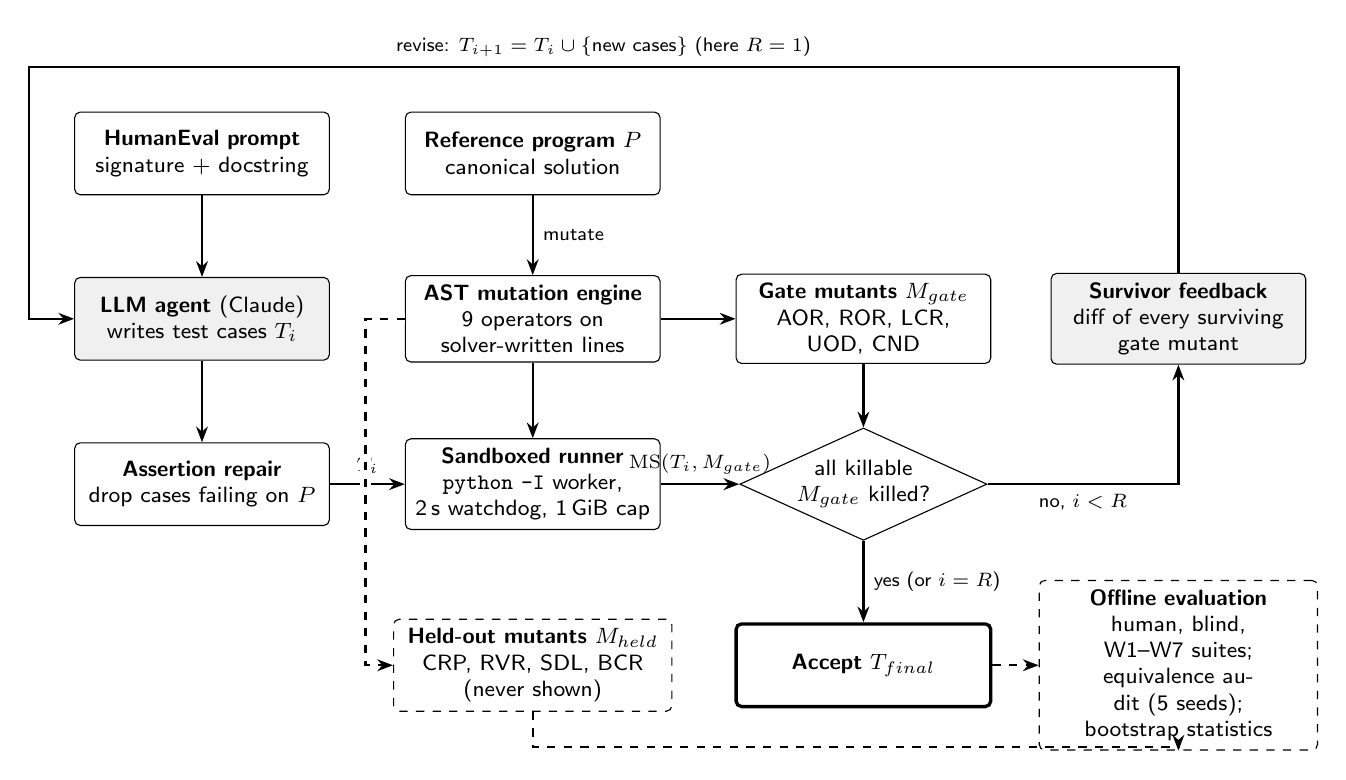
\begin{tikzpicture}[
  font=\sffamily\footnotesize,
  box/.style={draw, rounded corners=2pt, align=center, minimum height=1.05cm, text width=3.0cm, fill=white},
  agent/.style={box, fill=gray!12},
  off/.style={box, dashed, text width=3.3cm},
  dec/.style={draw, diamond, aspect=2.2, align=center, inner sep=0.5pt, fill=white},
  arr/.style={-{Stealth[length=2mm]}, thick},
  darr/.style={arr, dashed},
  gap/.style={preaction={draw, white, line width=4pt}},
  lab/.style={font=\sffamily\scriptsize, align=center}
]
% --- column 1: agent side
\node[box]   (prompt) at (0,4.2)  {\textbf{HumanEval prompt}\\signature + docstring};
\node[agent] (agent)  at (0,2.1)  {\textbf{LLM agent} (Claude)\\writes test cases $T_i$};
\node[box]   (repair) at (0,0)    {\textbf{Assertion repair}\\drop cases failing on $P$};
% --- column 2: program side
\node[box]   (prog)   at (4.2,4.2) {\textbf{Reference program} $P$\\canonical solution};
\node[box]   (mut)    at (4.2,2.1) {\textbf{AST mutation engine}\\9 operators on\\solver-written lines};
\node[box]   (run)    at (4.2,0)   {\textbf{Sandboxed runner}\\\texttt{python -I} worker,\\2\,s watchdog, 1\,GiB cap};
% --- column 3: gate
\node[box]   (gate)   at (8.4,2.1) {\textbf{Gate mutants} $M_{gate}$\\AOR, ROR, LCR, UOD, CND};
\node[dec]   (dec)    at (8.4,0)   {all killable\\$M_{gate}$ killed?};
\node[agent] (fb)     at (12.4,2.1) {\textbf{Survivor feedback}\\diff of every surviving\\gate mutant};
\node[box, very thick] (acc) at (8.4,-2.3) {\textbf{Accept} $T_{final}$};
% --- offline evaluation
\node[off]   (held)   at (4.2,-2.3) {\textbf{Held-out mutants} $M_{held}$\\CRP, RVR, SDL, BCR\\(never shown)};
\node[off]   (eval)   at (12.4,-2.3) {\textbf{Offline evaluation}\\human, blind, W1--W7 suites;\\equivalence audit (5 seeds);\\bootstrap statistics};

\draw[arr] (prompt) -- (agent);
\draw[arr] (agent) -- (repair);
\draw[arr] (prog) -- node[lab, right]{mutate} (mut);
\draw[arr] (mut) -- (gate);
\draw[arr] (mut) -- (run);
\draw[arr] (repair) -- node[lab, above]{$T_i$} (run);
\draw[arr] (run) -- node[lab, above]{$\mathrm{MS}(T_i,M_{gate})$} (dec);
\draw[arr] (gate) -- (dec);
\draw[arr] (dec) -- node[lab, right]{yes (or $i=R$)} (acc);
\draw[arr] (dec.east) -| node[lab, pos=0.25, below]{no, $i<R$} (fb.south);
\draw[arr] (fb.north) |- node[lab, pos=0.75, above]{revise: $T_{i+1}=T_i\cup\{\text{new cases}\}$ (here $R=1$)} (-2.2,5.3) |- (agent.west);
\draw[darr, gap] (mut.west) -- ++(-0.5,0) |- (held.west);
\draw[darr] (held.south) -- ++(0,-0.45) -| (eval.south);
\draw[darr] (acc) -- (eval);
\end{tikzpicture}%
}

\caption{MuGate workflow as implemented. Shaded boxes involve the LLM agent. Dashed elements are used only for offline evaluation and are never shown to the agent. In this study $P$ is the canonical solution and $R=1$.}\label{fig:workflow}
\end{figure}

% =====================================================================
\section{Experimental Setup}\label{sec:setup}

\paragraph{Data.} HumanEval~\cite{chen2021codex} provides 164 Python problems with prompt, canonical solution and human test function. We use a fixed uniform sample of \nTasks{} tasks drawn with seed 42 (Python's \texttt{random.sample}). The task list, the downloaded dataset's SHA-256 hash, and all agent prompts are part of the replication package.

\paragraph{Suites.} Human (the original HumanEval \texttt{check} function); agent vanilla (\casesVanillaKept{} cases); agent with blind augmentation (\blindCases{} further cases); agent after gate round~1 (\gateCases{} further cases); and W1--W7 applied to the vanilla cases.

\paragraph{Parameters.} Per-execution timeout 2\,s; audit budget 20\,s per mutant over all inputs; at most 400 audit inputs per task; audit seeds 0--4; bootstrap with $B=10\,000$ and seeds 0--4; $R=1$ feedback round.

\paragraph{Hardware and software.} All experiments ran on a laptop with an \cpuName{} CPU (2 cores, 2 threads), 3.4\,GB RAM and integrated graphics, under Windows~11 with CPython~3.12.10. The pipeline uses only the standard library; matplotlib~3.9.2 is used for figures. No GPU is used. The workload consists of interpreting thousands of short, branch-heavy Python programs in separate processes. Such work cannot be offloaded to a GPU and is dominated by interpreter start-up and per-call overhead, so process-level parallelism over CPU cores is the relevant scaling dimension, which we measure in Sect.~\ref{sec:rq3}. The test-writing agent ran as a hosted service, so no local accelerator was involved in generation either. A complete run (\nTasks{} tasks $\times$ 11 suites $\times$ \nMut{}+1 programs) took \evalWallMin{} minutes with two worker processes.

\paragraph{Metrics.} Adjusted mutation score (Eq.~\ref{eq:ms}); raw mutation score; gate and held-out scores and $\Delta_\gate$ (Eq.~\ref{eq:delta}); line coverage of the solver-written statements, measured with a trace function inside the worker; number of added cases; and wall-clock cost of the gate check.

% =====================================================================
\section{Results and Analysis}\label{sec:results}

\subsection{Mutants and Equivalence}
Table~\ref{tab:data} summarises the sample. Of the \casesAllRaw{} agent-written cases, \casesDropped{} (\repairRate\%) failed on $P$ and were removed by assertion repair: one expected \texttt{change\_base(0, 2)} to return \texttt{\textquotesingle 0\textquotesingle} (the reference returns an empty string, a case the docstring leaves open), and one assumed a sign convention for the unit digits of negative numbers in \texttt{multiply}. The mutation engine produced \nMut{} mutants (\nGateMut{} gate, \nHeldMut{} held-out); CRP alone accounts for almost half because HumanEval solutions contain many literal constants; no BCR mutant arose because no sampled solution uses \texttt{break} or \texttt{continue} in its solver-written lines. \nSurv{} mutants survived all four sound suites. The audit found no difference for \nEqAudit{} of them, a difference only on precondition-violating inputs for \nEqPre{} (e.g.\ a prime argument to \texttt{largest\_prime\_factor}, or duplicates where the docstring forbids them), and a valid distinguishing input for \nSurvKillable{}. These two killable survivors are genuine faults that \emph{no} suite detects, including the human one: a changed reset threshold in \texttt{minSubArraySum} (HumanEval/114) and a column wrap-around in \texttt{minPath} (HumanEval/129). The classification was identical for all five audit seeds.

\begin{table}[t]
\centering
\caption{Sample, agent cases and mutant statistics.}\label{tab:data}
\scriptsize
\begin{tabular}{@{}lr@{}}
\toprule
Statistic & Value\\
\midrule
HumanEval tasks in sample (seed 42) & 50 / 164\\
Agent cases written / kept after assertion repair (vanilla) & 266 / 265\\
Agent cases written / kept (blind augmentation) & 150 / 149\\
Agent cases written / kept (gate round 1) & 9 / 9\\
First-order mutants generated (all operators) & 883\\
\quad gate group (AOR, ROR, LCR, UOD, CND) & 282\\
\quad held-out group (CRP, RVR, SDL, BCR) & 601\\
Mutants surviving all four sound suites & 52\\
\quad equivalent (no difference on any audit input) & 36\\
\quad equivalent under the documented precondition & 14\\
\quad killable (valid distinguishing input found) & 2\\
Killable mutants (adjusted denominator) & 833 (94.3\%)\\
\bottomrule
\end{tabular}

\end{table}

\subsection{RQ1: Agent-Written versus Human Tests}
Table~\ref{tab:rq1} and Fig.~\ref{fig:ms} report the scores on the \nKillable{} killable mutants. Vanilla agent tests killed \killedVanilla{} (\msVanilla\%, CI \loVanilla--\hiVanilla), the human tests \killedHuman{} (\msHuman\%, CI \loHuman--\hiHuman). The difference of \dVanHum{} pp (paired CI \ciLoVanHum{} to \ciHiVanHum) is not significant (Wilcoxon $p=\pWVanHum$, sign test $p=\pSVanHum$). The suites are not nested: \onlyBVanHum{} mutants are killed only by the human tests and \onlyAVanHum{} only by the agent tests. Agent tests were perfect on \perfectVanilla{} tasks, human tests on \perfectHuman. H1 is therefore not supported at this sample size; on short, well-specified functions an LLM agent writes tests of roughly human-reference strength.

\begin{table}[t]
\centering
\caption{RQ1 and RQ3: mutation-detection strength per suite on \nKillable{} killable mutants of \nTasks{} tasks. CI: task-level cluster bootstrap. Line cov.: mean coverage of solver-written statements. Perfect: tasks with adjusted MS of 100\%.}\label{tab:rq1}
\scriptsize
\setlength{\tabcolsep}{3.5pt}
\begin{tabular}{@{}lrrrrrrr@{}}
\toprule
Suite & Cases & Killed & Adj.\ MS (\%) & 95\% CI & Raw MS & Line cov. & Perfect\\
 &  & /833 &  & (bootstrap) & (\%) & (\%) & tasks\\
\midrule
Human (reference) & -- & 813 & 97.6 & [95.6, 99.1] & 92.1 & 99.8 & 39/50\\
Agent, vanilla & 265 & 802 & 96.3 & [93.3, 99.0] & 90.8 & 99.8 & 41/50\\
Agent, +blind & 414 & 819 & 98.3 & [96.6, 99.7] & 92.8 & 99.8 & 45/50\\
Agent, +gate R1 & 274 & 813 & 97.6 & [94.8, 99.5] & 92.1 & 99.8 & 42/50\\
\bottomrule
\end{tabular}

\end{table}

\begin{figure}[t]
\centering
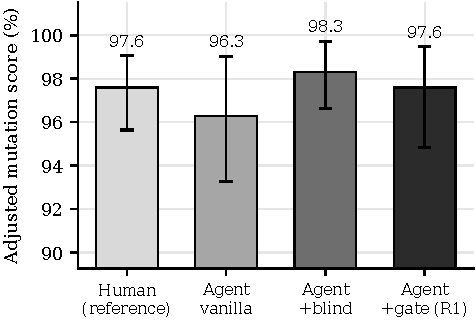
\includegraphics[width=0.62\textwidth]{figures/fig2_ms_by_suite.pdf}
\caption{Adjusted mutation score per suite with 95\% task-level bootstrap confidence intervals.}\label{fig:ms}
\end{figure}

\paragraph{Coverage is not strength.} Following MutGen~\cite{wang2025mutgen}, we compared line coverage with mutation score. All four sound suites cover \covMean\% of solver-written statements on average (\covFull{} of \nTasks{} tasks fully), yet \nFullCovImperfect{} tasks reach full coverage with an imperfect vanilla mutation score, the worst being \worstTask{} at \worstMS\%. Across tasks, coverage and mutation score are uncorrelated (Pearson $r=\pearsonCovMs$; Fig.~\ref{fig:cov}). The direction of MutGen's finding thus replicates in Python; the magnitude is smaller because HumanEval functions are short and leave little code unexercised.

\begin{figure}[t]
\centering
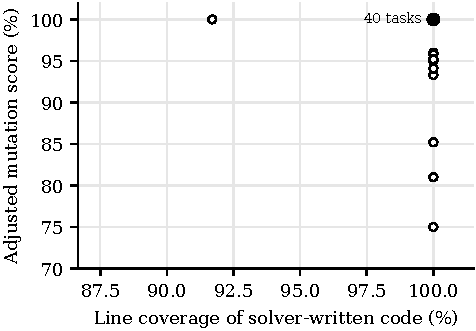
\includegraphics[width=0.55\textwidth]{figures/fig6_coverage_vs_ms.pdf}
\caption{Per-task line coverage versus adjusted mutation score of the vanilla agent suite. Nearly all tasks are fully covered while mutation scores vary.}\label{fig:cov}
\end{figure}

\subsection{RQ2: Test-Weakness Patterns}
Table~\ref{tab:rq2} and Fig.~\ref{fig:weak} show that every weakening removes most of the suite's strength although W1--W4 execute exactly the same calls as the sound suite. Exception swallowing (W4) is nearly as bad as not testing at all (\msWFour\%), because it also hides crashes. No-oracle and tautological assertions (W1, W2) keep only crash and timeout detection (\msWOne\% and \msWTwo\%). A type-only oracle (W3) keeps somewhat more (\msWThree\%), because many mutants change the result type (e.g.\ to \texttt{None}). Deleting all but one case (W5) is the mildest weakening (\msWFive\%) because the remaining case is still sound. W6 and W7 score 0\% by construction. H2 is supported: weakening the oracle removes far more strength than removing test cases, and coverage cannot reveal the difference.

\begin{table}[t]
\centering
\caption{RQ2: adjusted and raw mutation scores of the seven weakening operators applied to the vanilla agent cases.}\label{tab:rq2}
\scriptsize
\begin{tabular}{@{}llrr@{}}
\toprule
ID & Transformation of the sound vanilla cases & Adj.\ MS (\%) & Raw MS (\%)\\
\midrule
-- & none (sound vanilla suite) & 96.3 & 90.8\\
W5 & Test deletion (keep first case only) & 67.5 & 63.6\\
W3 & Type-only oracle (assert isinstance(f(x), T)) & 31.8 & 30.0\\
W2 & Tautological oracle (assert f(x) $==$ f(x)) & 22.3 & 21.1\\
W1 & No-oracle (call, then assert True) & 22.2 & 21.0\\
W4 & Exception-swallowing (try/except Exception: pass) & 3.4 & 3.2\\
W6 & Skipped tests (dead if False: branch) & 0.0 & 0.0\\
W7 & Mocked-out logic (stub returns expected value) & 0.0 & 0.0\\
\bottomrule
\end{tabular}

\end{table}

\begin{figure}[t]
\centering
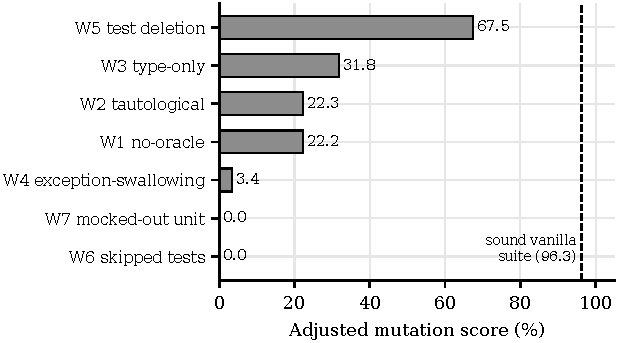
\includegraphics[width=0.62\textwidth]{figures/fig4_weakening.pdf}
\caption{Adjusted mutation score under the seven weakening operators; dashed line: the sound vanilla suite.}\label{fig:weak}
\end{figure}

\subsection{RQ3: Survivor Feedback, Generalisation and Cost}\label{sec:rq3}
After the vanilla run, \survShown{} gate mutants in \tasksShown{} tasks survived and were shown to the agent. The agent judged 9 of them equivalent and targeted the other 9 with \gateCases{} new cases in \tasksRevised{} tasks (\gateCasesPerTask{} per task). According to the audit, only \survShownKillable{} of the shown survivors were killable, and the round killed all \survShownKilled{}. The gate-group score therefore reached \msGateGrpGate\% (Table~\ref{tab:heldout}). One of the agent's added cases rested on a misreading of the code and targeted a mutant that the audit later classified as equivalent, which illustrates that survivor diffs expose implementation details the agent may misinterpret.

\begin{table}[t]
\centering
\caption{Gate-group versus held-out scores (adjusted). $\Delta_{gate}$ as in Eq.~\ref{eq:delta}; negative values mean held-out mutants are harder.}\label{tab:heldout}
\scriptsize
\begin{tabular}{@{}lrrr@{}}
\toprule
Suite & Gate MS (\%) & Held-out MS (\%) & $\Delta_{gate}$ (pp)\\
 & (/271) & (/562) & \\
\midrule
Human (reference) & 98.2 & 97.3 & \ensuremath{-0.8}\\
Agent, vanilla & 97.4 & 95.7 & \ensuremath{-1.7}\\
Agent, +blind & 98.2 & 98.4 & \ensuremath{+0.2}\\
Agent, +gate R1 & 100.0 & 96.4 & \ensuremath{-3.6}\\
\bottomrule
\end{tabular}

\end{table}

\begin{figure}[t]
\centering
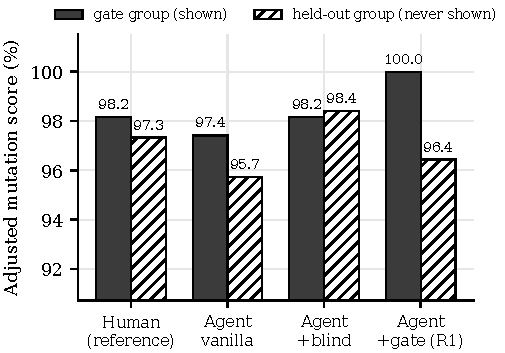
\includegraphics[width=0.62\textwidth]{figures/fig3_gate_vs_heldout.pdf}
\caption{Gate-group (shown) and held-out (never shown) adjusted mutation scores. Feedback closes the gate group completely but moves the held-out score only slightly.}\label{fig:heldout}
\end{figure}

On the held-out mutants, the score moved only from \msHeldGrpVanilla\% to \msHeldGrpGate\% (Fig.~\ref{fig:heldout}), and $\Delta_\gate$ fell from \deltaVanilla{} to \deltaGate{} pp, i.e.\ the gap \emph{widened}. Overall, the gated suite gained \dGatVan{} pp over vanilla (CI \ciLoGatVan{} to \ciHiGatVan; Wilcoxon $p=\pWGatVan$; \upGatVan{} tasks improved, none worsened). Unguided augmentation with three extra cases per task gained \dBliVan{} pp (CI \ciLoBliVan{} to \ciHiBliVan; \upBliVan{} tasks improved, none worsened; sign test $p=\pSBliVan$), the only improvement whose interval excludes zero. The difference between blind and gated suites is not significant (Table~\ref{tab:cmp}). Per added case, feedback was far more efficient: \gateCases{} feedback cases killed \onlyAGatVan{} additional mutants, whereas \blindCases{} blind cases killed \onlyABliVan. H3 is not supported: on this benchmark one feedback round strengthened the suite locally but did not measurably generalise.

\begin{table}[t]
\centering
\caption{Paired comparisons of adjusted mutation score (pp = percentage points). Tasks +/$-$: tasks where the first suite scores higher/lower.}\label{tab:cmp}
\scriptsize
\begin{tabular}{@{}lrrrrr@{}}
\toprule
Comparison & $\Delta$ MS (pp) & 95\% CI (pp) & Tasks +/$-$ & Wilcoxon $p$ & Sign $p$\\
\midrule
Vanilla $-$ Human & \ensuremath{-1.3} & [\ensuremath{-4.7}, \ensuremath{+1.8}] & 5/3 & 0.624 & 0.727\\
Blind $-$ Vanilla & \ensuremath{+2.0} & [\ensuremath{+0.3}, \ensuremath{+4.3}] & 6/0 & 0.036 & 0.031\\
Gate R1 $-$ Vanilla & \ensuremath{+1.3} & [\ensuremath{0.0}, \ensuremath{+3.0}] & 3/0 & 0.181 & 0.250\\
Gate R1 $-$ Blind & \ensuremath{-0.7} & [\ensuremath{-3.3}, \ensuremath{+1.5}] & 2/5 & 0.447 & 0.453\\
Gate R1 $-$ Human & \ensuremath{0.0} & [\ensuremath{-3.4}, \ensuremath{+3.0}] & 6/3 & 0.193 & 0.508\\
\bottomrule
\end{tabular}

\end{table}

\paragraph{Cost.} Table~\ref{tab:rq3} reports the cost on this machine. Running the agent's suite once on $P$, as an ungated pipeline does, took \costBase\,s per task, dominated by starting one interpreter. Checking all gate mutants in one warm worker took \costBatched\,s per task (\costOverBase$\times$ the ungated cost, including the 2-second timeouts of looping mutants). Starting a fresh interpreter for every mutant took \costIsolated\,s, \costRatio$\times$ slower than batching. A single suite execution inside a warm worker has a median duration of \execMedianMs\,ms, so process start-up, not test execution, dominates. Running all \nMut{} mutants against the human suite took \scaleOne\,s with one worker and \scaleTwo\,s with two (speed-up \speedup), confirming that the workload scales with CPU processes rather than requiring specialised hardware.

\begin{table}[t]
\centering
\caption{RQ3: effort and cost of one feedback round (times are means over three repetitions on the hardware in Sect.~\ref{sec:setup}).}\label{tab:rq3}
\scriptsize
\begin{tabular}{@{}lr@{}}
\toprule
Quantity & Value\\
\midrule
Tasks with $\geq$1 surviving gate mutant shown & 11 / 50\\
Surviving gate mutants shown to the agent & 18\\
\quad of which killable (non-equivalent) & 7\\
\quad of which killed after round 1 & 7\\
Tasks in which the agent added cases & 4 / 50\\
Cases added in round 1 (total / per task) & 9 / 0.18\\
Cases added by blind augmentation (total) & 149\\
Suite run on $P$ only, mean per task (s) & 0.158\\
Gate check, warm batched worker, mean per task (s) & 0.670\\
Gate check, one interpreter per mutant, mean per task (s) & 2.173\\
Median single suite execution inside the worker (ms) & 0.63\\
\bottomrule
\end{tabular}

\end{table}

\subsection{Operator-Level View and Robustness}
Figure~\ref{fig:ops} shows survival per operator. For every suite, constant-replacement (CRP) mutants make up most of the surviving killable mutants: 22 of 31 for the vanilla suite, and all 20 remaining survivors after the gate round, which never saw a CRP mutant. Off-by-one constants in loop bounds and thresholds are exactly the faults that boundary-value inputs expose, and the blind cases, which added such inputs, left only 8 CRP survivors. A second complete evaluation run reproduced 10\,261 of the 10\,263 kill statuses. The two differences occurred in weakened suites (W2, W5) on mutants whose run time is close to the 2-second limit, so they depend on machine load. All sound-suite results, coverage values and mutants were identical, and the largest effect on any reported score is 0.1 pp (W2). The equivalence classification was identical for all five audit seeds, and the bootstrap interval endpoints varied by at most 0.2 pp across five bootstrap seeds. The only stochastic input that was not repeated is the agent itself (Sect.~\ref{sec:threats}).

\begin{figure}[t]
\centering
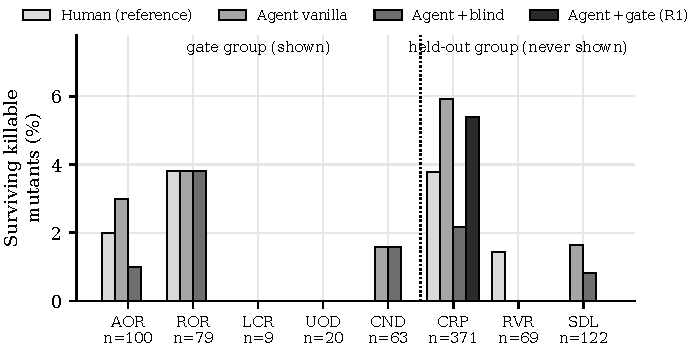
\includegraphics[width=\textwidth]{figures/fig5_survival_by_operator.pdf}
\caption{Share of killable mutants that survive, per operator and suite ($n$ = killable mutants per operator; BCR is omitted because the sample contains no BCR mutant).}\label{fig:ops}
\end{figure}

% =====================================================================
\section{Discussion}\label{sec:discussion}

\paragraph{Agent tests are close to human tests on HumanEval.} On short, well-specified functions, prompt-only tests from a current LLM agent are statistically indistinguishable from the benchmark's human tests in mutation score. The two suites miss different mutants, so the agent's tests are a complement rather than a replacement. That two genuine faults escape \emph{all} suites, including the reference, agrees with EvalPlus's observation that HumanEval's tests are insufficient~\cite{liu2023evalplus}.

\paragraph{Feedback is precise but local.} Survivor feedback is the most case-efficient intervention we measured, but its gains were confined to the mutants it exposed. The held-out score rose by less than one point and the held-out gap widened. Part of this is structural: our operator-based split puts most constant-replacement mutants in the held-out group, and the fault types differ. Mutation-guided pipelines that report gains on the same mutants they used for guidance~\cite{wang2025mutgen,chang2026advertest} may therefore overstate generalisation; a held-out mutant set is a cheap safeguard.

\paragraph{More tests helped more than targeted tests.} Three extra unguided cases per task gave the largest and only statistically supported gain. On HumanEval, the main weakness of the agent's tests was too few probing inputs rather than wrong expectations, and broad augmentation reaches more fault types than mutant-specific fixes. A practical gate could combine both: require a minimum number of diverse cases, then use survivor feedback for the remainder.

\paragraph{Weak oracles are the real risk.} The weakening results show that oracle quality, not test count or coverage, determines strength. A suite that swallows exceptions or asserts only tautologies passes on almost every faulty program while looking identical in coverage reports. Mutation score detects these patterns immediately, which supports using it as an acceptance signal for agent-written tests, as reward-hacking studies motivate~\cite{gabor2025evilgenie,zhao2026specbench}.

% =====================================================================
\section{Threats to Validity and Limitations}\label{sec:threats}

\paragraph{Construct validity.} Mutation score is a proxy for real-fault detection~\cite{just2014mutants}. Our operators are syntactic and first-order, so semantic or multi-location faults are not represented~\cite{hort2025semantic}. The audit compares return values and exception types only. A mutant that differs only by a side effect, such as removing the defensive copy \texttt{l = list(l)} in HumanEval/33 so that the caller's list is modified, is classified as equivalent. The precondition labels for \nEqPre{} survivors are manual judgements; they are documented individually and affect the denominator by at most \nEqPre{} of \nKillable{} mutants.

\paragraph{Internal validity.} The same LLM (Claude) wrote the pipeline and the agent tests. Blinding was procedural: the agent saw only the prompt file when writing vanilla and blind cases and only the survivor file in round 1, but it designed the study and had read an earlier draft that discussed an edge case of HumanEval/40, which may have influenced one blind case. HumanEval is public and likely present in the model's training data, which may inflate the vanilla scores. Each suite was written once, so sampling variance of the agent is not captured. Blind cases were written in the same sitting as the vanilla cases rather than by a separate request. Only one feedback round was run, and the gate decision was not automated, because equivalent survivors make a fully automatic 100\% threshold unattainable without an equivalence oracle. The gate/held-out split confounds feedback exposure with operator type.

\paragraph{External validity.} The study covers \nTasks{} of 164 HumanEval tasks, one language, one agent and function-level code with known-correct reference programs. Results may differ for repository-scale tasks, where coverage is lower and hacking gaps larger~\cite{zhao2026specbench}, and for agents that write both the patch and the tests.

\paragraph{Conclusion validity.} With 50 tasks and many tasks at 100\%, the paired tests have few non-zero differences (3--9 per comparison) and low power. Non-significant differences, including vanilla versus human, should be read as inconclusive.

% =====================================================================
\section{Conclusion and Future Work}\label{sec:conclusion}

We presented MuGate, a sandboxed, standard-library mutation-analysis pipeline for agent-written Python tests with a shown/held-out mutant split and a suite-independent equivalence audit, and used it on \nTasks{} HumanEval tasks. \textbf{RQ1:} prompt-only tests from an LLM agent reached \msVanilla\% adjusted mutation score against \msHuman\% for human tests, a difference that was not significant, while coverage was near-complete and uninformative. \textbf{RQ2:} oracle weakenings cut mutation score to \msWFour--\msWThree\% at identical coverage, whereas deleting cases kept \msWFive\%. \textbf{RQ3:} one round of survivor feedback killed every killable mutant it exposed with only \gateCases{} added cases, but did not measurably improve the held-out score. Unguided augmentation gave the only statistically supported gain, at a much higher case count. A gate check costs a fraction of a second per task on a two-core laptop CPU, and no GPU is needed.

Future work should (i) run several agents and repeated generations to capture model variance, (ii) use multiple feedback rounds and a random rather than operator-based held-out split to separate exposure from fault type, (iii) add semantic and higher-order mutants and side-effect-aware equivalence checking, and (iv) move to repository-level tasks in which the agent writes both the patch and the tests.

\paragraph{Data availability.} The pipeline, agent prompts and cases, raw results and all scripts that generate the tables and figures are publicly available at \url{https://github.com/gondalmahnoor78-a11y/mugate-humaneval}.

\bibliographystyle{splncs04}
\bibliography{refs}

\end{document}
